\newpage

\section{Diseño lógico}
\label{sec:diseno-logico}

En esta sección se describe la transformación del modelo entidad-relación extendido en un esquema relacional, trabajada en la Práctica~3. Se presentan el inventario del que partió la transformación, las decisiones de tipos de dato, la forma en que se aplicó cada regla, el esquema resultante y la revisión de que este conserva el significado del modelo.

\subsection{Inventario del modelo extendido}

Antes de aplicar las reglas se levantó un inventario de los elementos del modelo extendido, porque cada tipo de elemento se transforma con una regla distinta y omitir uno habría dejado una parte del negocio sin representar. La Tabla~\ref{tab:inventario} resume ese inventario.

\begin{table}[H]
    \centering
    \small
    \begin{tabular}{lc}
        \toprule
        \textbf{Elemento} & \textbf{Cantidad} \\
        \midrule
        Entidades fuertes & 8 \\
        Entidades débiles & 2 \\
        Subclases de la jerarquía de Usuario & 3 \\
        Relaciones binarias uno a muchos & 14 \\
        Relaciones binarias muchos a muchos & 2 \\
        Relaciones ternarias & 1 \\
        Atributos multivaluados & 1 \\
        Atributos compuestos & 5 \\
        Atributos derivados & 7 \\
        Atributos de relación & 3 \\
        \bottomrule
    \end{tabular}
    \captionsetup{labelfont=bf, textfont=it, labelsep=newline, justification=raggedright, singlelinecheck=false}
    \caption{Inventario del modelo entidad-relación extendido}
    \label{tab:inventario}
\end{table}

\subsection{Tipos de dato}

Para no justificar cada columna por separado, se fijó primero el tipo que recibe cada clase de atributo, como se muestra en la Tabla~\ref{tab:tipos}. El criterio general fue elegir el tipo que valida el dato por sí mismo: un tipo de fecha rechaza el 31 de febrero y un decimal exacto evita que las sumas de dinero acumulen errores de redondeo, como ocurriría con los tipos de punto flotante.

\begin{table}[H]
    \centering
    \small
    \begin{tabularx}{\textwidth}
        {
            >{\RaggedRight\arraybackslash}p{3.6cm}
            >{\RaggedRight\arraybackslash}p{4.2cm}
            >{\RaggedRight\arraybackslash}X
        }
        \toprule
        \textbf{Clase de atributo} & \textbf{Tipo en PostgreSQL} & \textbf{Razón} \\
        \midrule
        Identificadores & \texttt{INTEGER} con identidad & El gestor asigna el siguiente número y permite cargar números conocidos. \\
        Claves parciales & \texttt{SMALLINT} & Se reinician en cada evento y nunca son grandes. \\
        Dinero & \texttt{NUMERIC(10,2)} & Decimal exacto a centavos. \\
        Cantidades de inventario & \texttt{NUMERIC(10,3)} & Decimal exacto en gramos, mililitros o piezas. \\
        Listas cerradas & \texttt{VARCHAR} con \texttt{CHECK} & La lista queda visible y puede ampliarse. \\
        Fechas e instantes & \texttt{DATE} y \texttt{TIMESTAMPTZ} & Validan la fecha y guardan el instante exacto. \\
        Contraseñas & \texttt{VARCHAR(255)} & Solo se guarda su \textit{hash}, nunca el texto. \\
        \bottomrule
    \end{tabularx}
    \captionsetup{labelfont=bf, textfont=it, labelsep=newline, justification=raggedright, singlelinecheck=false}
    \caption{Tipos de dato por clase de atributo}
    \label{tab:tipos}
\end{table}

\subsection{Aplicación de las reglas de transformación}

La transformación siguió las nueve reglas descritas en el marco teórico \parencite[p.~289]{elmasri_navathe}. En algunos casos fue necesario interpretar la regla para no perder una propiedad del modelo; esas decisiones se explican a continuación.

\subsubsection{Entidades, atributos compuestos y multivaluados}

Las ocho entidades fuertes produjeron ocho tablas, cada una con su identificador como clave primaria. Los cinco atributos compuestos son todos de fecha u hora, y el cliente los consulta por sus componentes; aplicar la regla al pie de la letra, guardando el día, el mes y el año como columnas sueltas, habría permitido guardar fechas imposibles. Por ello, la fecha se guarda con el tipo nativo del gestor, que la valida, y cada componente es una columna generada que el gestor calcula y que nadie puede escribir, de modo que nunca contradice a la fecha. El único atributo multivaluado, los organizadores del evento, se llevó a una tabla propia cuya clave combina el evento y el organizador.

Los atributos derivados no se guardan, porque una copia de un dato calculado debe mantenerse sincronizada y, si alguna vez no se actualiza, la base tiene dos versiones distintas de lo mismo. En su lugar, se calculan en vistas: el número de mesas del evento, el total acumulado y el saldo de cada cuenta, la edad de cada usuario, las propinas acumuladas de cada mesero y la disponibilidad de cada producto. El precio cobrado de una comanda, en cambio, sí se guarda, porque es el precio que tenía el producto al momento del pedido y no debe cambiar aunque el catálogo cambie después.

\subsubsection{Relaciones}

Las catorce relaciones uno a muchos se representaron con una clave foránea en la tabla del lado de muchos, y su participación mínima se expresó con \texttt{NOT NULL} cuando es obligatoria. Las dos relaciones muchos a muchos, \textit{Receta} e \textit{Incluye}, produjeron las tablas \texttt{receta} y \texttt{paquete\_producto}, cuyas claves combinan las de las dos entidades y que conservan los atributos de la relación, como la cantidad por porción.

La relación ternaria \textit{Acuerda} produjo la tabla \texttt{acuerdo}, cuya clave primaria combina las claves del evento, del paquete y del producto, porque ningún par de ellas determina al tercero. Esta tabla no tiene una clave foránea hacia \texttt{paquete\_producto}: el contenido del paquete es una base y no una lista cerrada, y esa clave haría que el gestor rechazara justamente lo que el negocio permite, acordar en un evento un producto que el paquete no traía.

\subsubsection{Entidades débiles}

Mesa y Cuenta dependen del evento por identificación, así que sus tablas llevan una clave primaria compuesta por el número de evento y su clave parcial. De esta forma, la mesa tres de un evento y la de otro son filas distintas, y el gestor rechaza una segunda mesa tres en el mismo evento. Su clave foránea hacia el evento borra en cascada, porque una mesa o una cuenta no tienen sentido sin su evento; sin embargo, esa cascada se detiene si el evento ya tiene comandas, pagos o anticipos, cuyas claves impiden el borrado para conservar el historial del dinero.

\subsubsection{Jerarquía de Usuario}

Para la jerarquía se eligió la estrategia de una tabla para la superclase y una para cada subclase. Aunque las subclases tienen pocos atributos propios, lo que decidió la estrategia fueron sus relaciones: seis relaciones solo admiten a usuarios de una subclase, como la propina, que solo puede ir a un mesero, y eso exige que la clave foránea apunte a la tabla \texttt{mesero} y no a \texttt{usuario}. Con una sola tabla para toda la jerarquía, el gestor aceptaría una propina para un cocinero; y sin la tabla de la superclase, los datos comunes se repetirían en tres tablas y el nombre de acceso no podría ser único entre todas ellas.

La restricción disjunta se hace cumplir de forma declarativa: la tabla \texttt{usuario} guarda un discriminador \texttt{rol}, cada subclase lo repite fijo a su valor y apunta a \texttt{usuario} con una clave foránea de dos columnas, el identificador y el rol, de modo que un usuario no puede aparecer en dos subclases. La restricción total se verifica con un disparador diferido que, al confirmar la transacción, comprueba que cada usuario tenga su fila en la subclase que corresponde a su rol.

\subsection{Esquema resultante}

La transformación produjo diecisiete tablas y seis vistas, que se listan en la Tabla~\ref{tab:tablas} junto con el elemento del modelo del que provienen. La Figura~\ref{fig:diagrama-relacional} muestra el diagrama relacional, en el que se distinguen la clave primaria, las claves foráneas y las columnas generadas de cada tabla.

\begin{table}[H]
    \centering
    \small
    \begin{tabularx}{\textwidth}
        {
            >{\RaggedRight\arraybackslash}p{3.4cm}
            >{\RaggedRight\arraybackslash}X
        }
        \toprule
        \textbf{Tabla} & \textbf{Origen en el modelo extendido} \\
        \midrule
        \texttt{evento} & Entidad fuerte Evento \\
        \texttt{evento\_organizador} & Atributo multivaluado de Evento \\
        \texttt{usuario} & Superclase Usuario \\
        \texttt{mesero}, \texttt{bar\_cocina}, \texttt{cajero\_admin} & Subclases de Usuario \\
        \texttt{mesa}, \texttt{cuenta} & Entidades débiles, con las relaciones \textit{Atiende} y \textit{Tiene} \\
        \texttt{producto} & Entidad fuerte Producto, con la relación \textit{Variante} \\
        \texttt{ingrediente}, \texttt{paquete} & Entidades fuertes \\
        \texttt{receta}, \texttt{paquete\_producto} & Relaciones muchos a muchos \textit{Receta} e \textit{Incluye} \\
        \texttt{acuerdo} & Relación ternaria \textit{Acuerda} \\
        \texttt{comanda} & Entidad fuerte Comanda, con \textit{Genera}, \textit{Levanta}, \textit{Referencia}, \textit{Prepara} y \textit{Cancela} \\
        \texttt{pago} & Entidad fuerte Pago, con \textit{Recibe}, \textit{Maneja} y \textit{Recibe propina} \\
        \texttt{anticipo} & Entidad fuerte Anticipo, con \textit{Recibe} \\
        \bottomrule
    \end{tabularx}
    \captionsetup{labelfont=bf, textfont=it, labelsep=newline, justification=raggedright, singlelinecheck=false}
    \caption{Tablas del esquema relacional}
    \label{tab:tablas}
\end{table}

\begin{figure}[p]
    \centering
    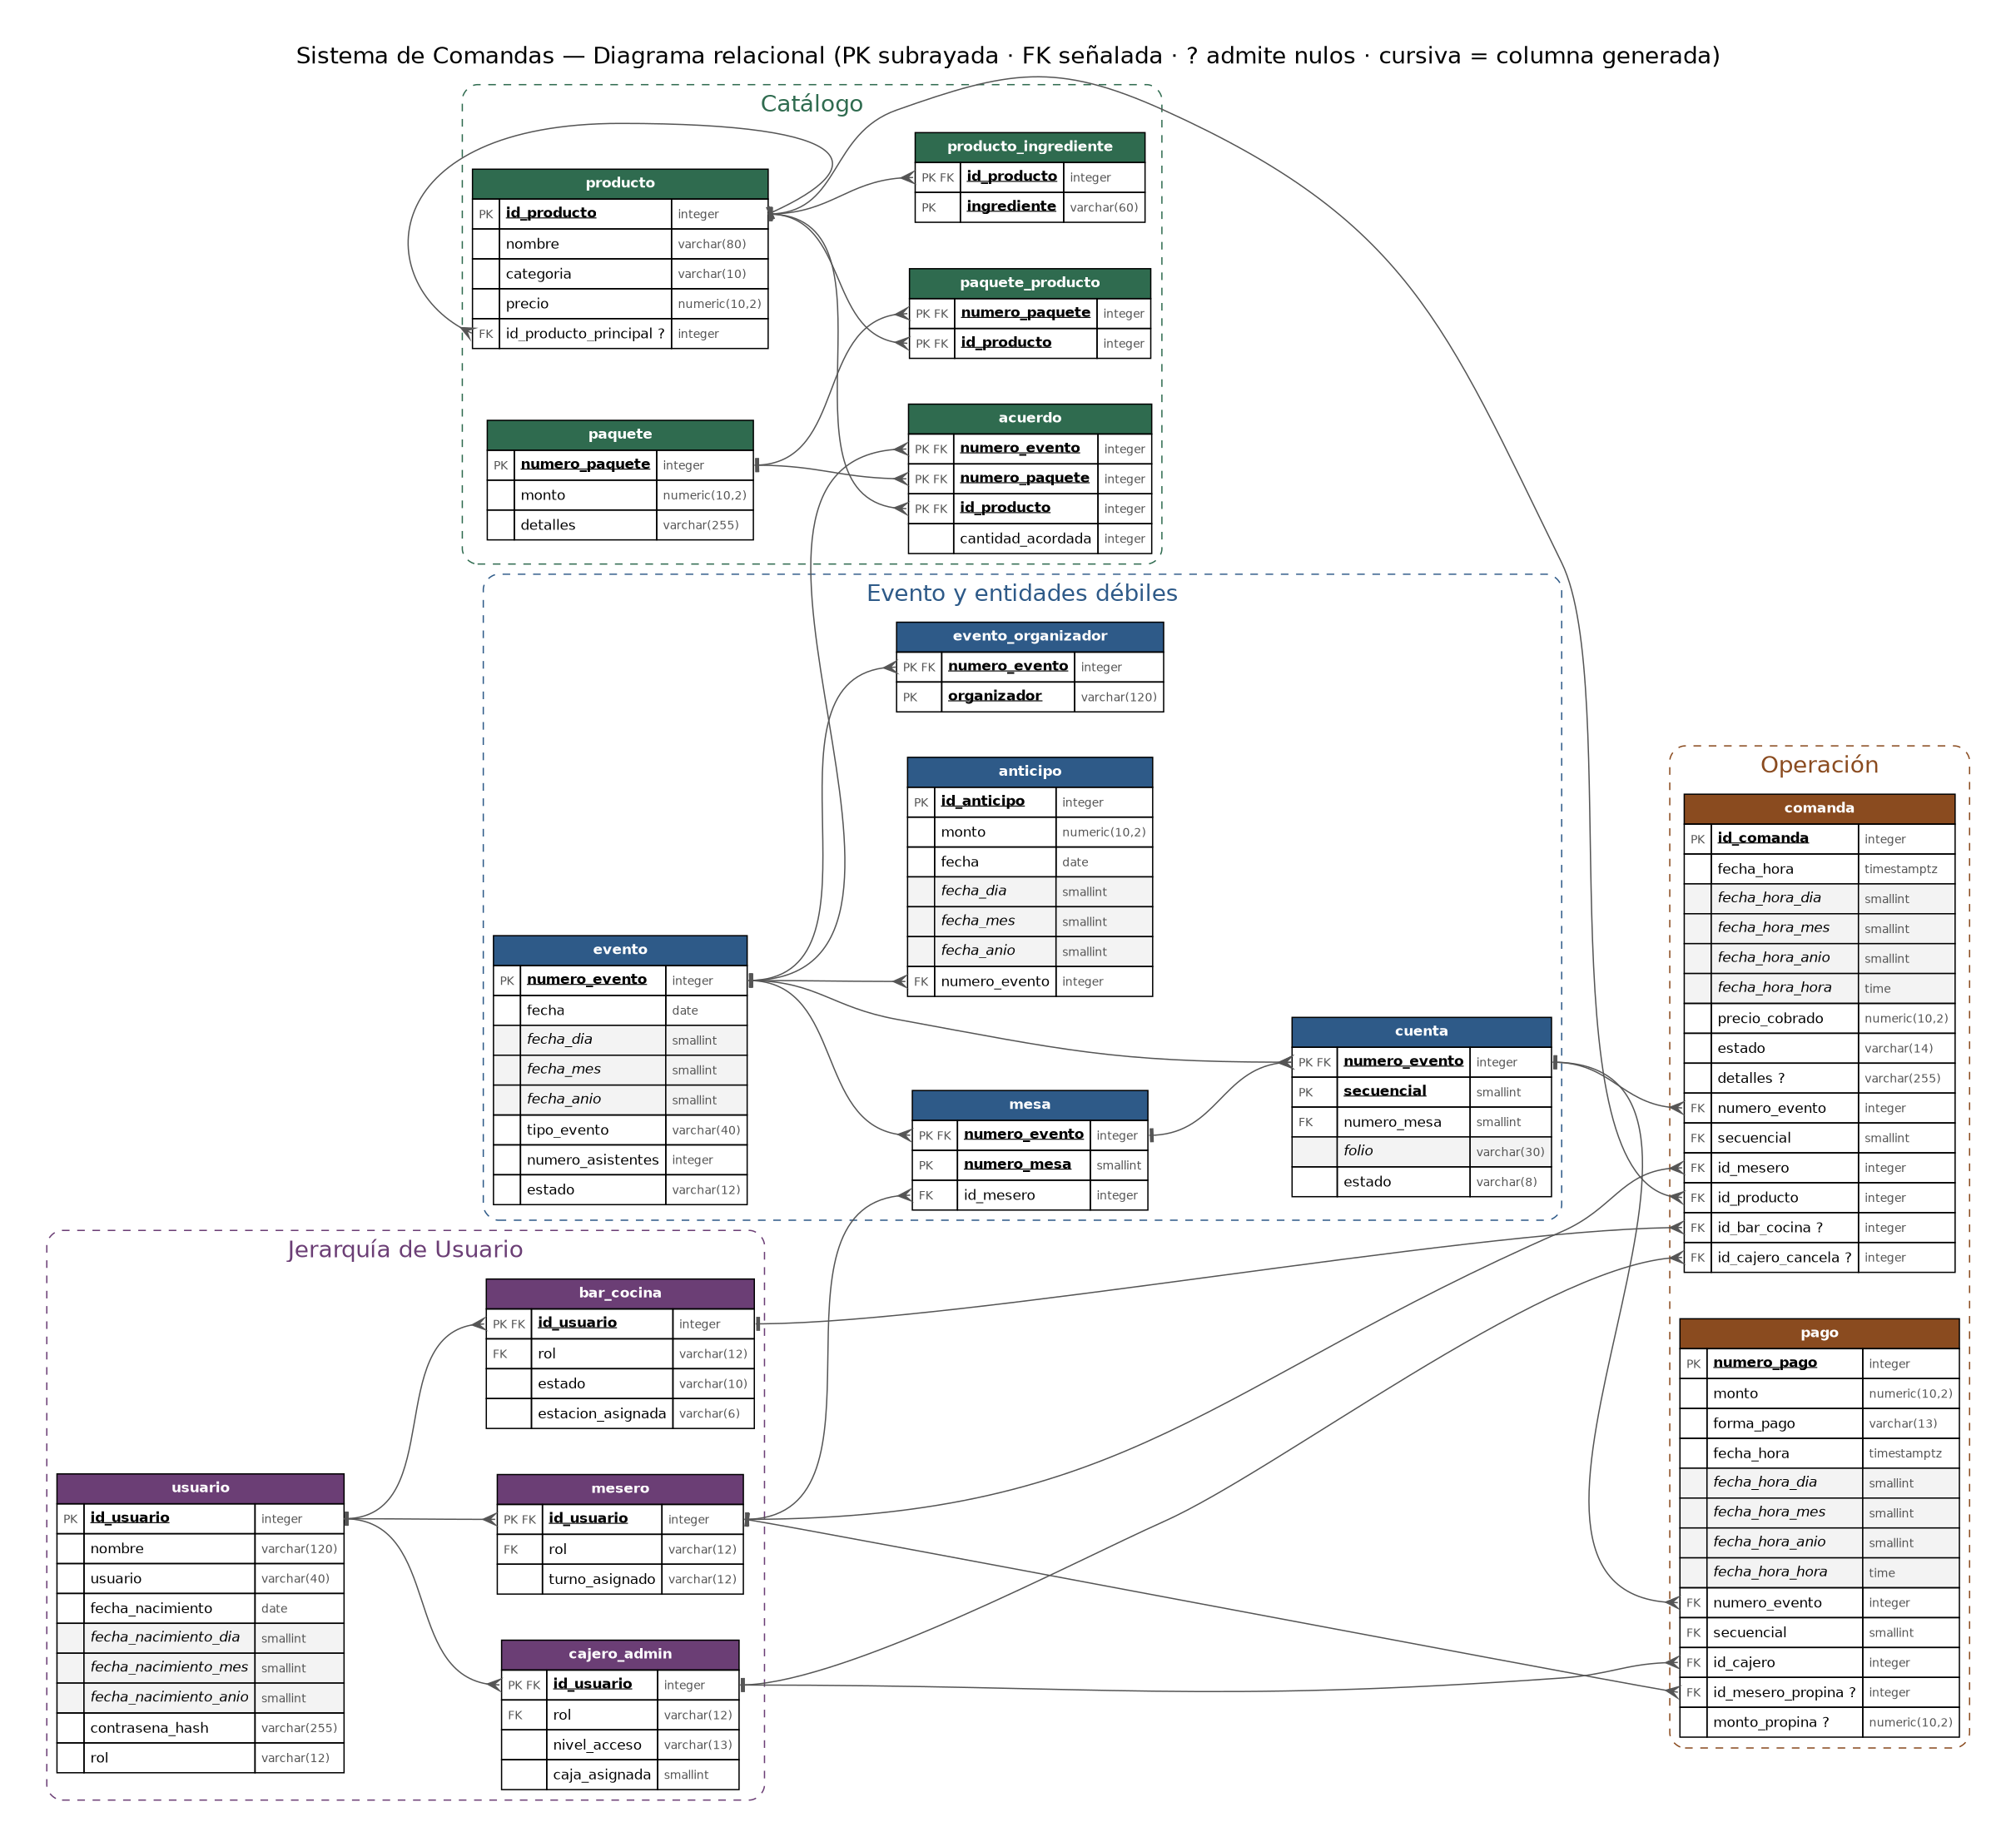
\includegraphics[width=\linewidth, height=0.85\textheight, keepaspectratio]{../../modelo/diagrama-relacional.png}
    \captionsetup{labelfont=bf, textfont=it, labelsep=newline, justification=raggedright, singlelinecheck=false}
    \caption{Diagrama relacional del sistema de comandas}
    \label{fig:diagrama-relacional}
\end{figure}

En total, el esquema tiene noventa y siete columnas y veinticinco claves foráneas. El diccionario de datos, con el tipo, las restricciones y la descripción de cada columna, se encuentra en el repositorio del proyecto.

\subsection{Preservación del significado}

Una vez ejecutado el esquema, se revisó contra el inventario, elemento por elemento, que conservara el significado del modelo extendido. Las ocho entidades fuertes, las dos débiles y las tres subclases tienen su tabla, y cada relación quedó expresada con restricciones: el máximo de uno, en la tabla donde vive la clave foránea; el máximo de muchos, en que esa columna no es única; y el mínimo, en que la columna sea obligatoria o admita nulos.

Algunas reglas no se hacen cumplir en el esquema, y se dejaron documentadas para que las valide la aplicación. Que todo evento tenga al menos una mesa y todo producto al menos un ingrediente no se exige, porque el evento se registra semanas antes de montar las mesas y la receta se captura después de dar de alta el producto; el número máximo de mesas depende del acomodo del salón; y que el mesero que recibe la propina sea quien atendió la mesa no es una regla, porque un mesero puede cubrir a otro.

La única regla del modelo extendido que no se preservó es el cambio de rol conservando el historial. Como la clave foránea de cada subclase incluye el rol, el gestor impide cambiar el rol de un usuario que ya tiene registros, de modo que el historial queda protegido, pero el cambio de puesto requiere un procedimiento administrativo. Se aceptó esta limitación porque la disyunción es la regla que sostiene el control del dinero y el cambio de rol es un evento poco frecuente; si llegara a ser común, la solución sería separar la identidad de la persona del rol que desempeña en cada periodo.
